%\documentclass[12pt]{article}
%\usepackage[a4paper, margin=1in]{geometry} 
%\usepackage{graphicx} 
%\usepackage{hyperref}
%\usepackage{float}
%\usepackage{multicol}
%\usepackage{multirow}
%\usepackage[font=small, labelfont=bf]{caption}
%
%\begin{document}

%
% Statistical analysis
%
\subsection{Statistical analysis}
Statistical tests are performed to give an explanation to observed alignment scores.

%
% Hypothesis testing
%
\subsubsection*{Hypothesis testing} 
\begin{itemize}
\item Alternative hypothesis
\item Null hypothesis
\end{itemize}

\begin{figure}[H]
  \centering
      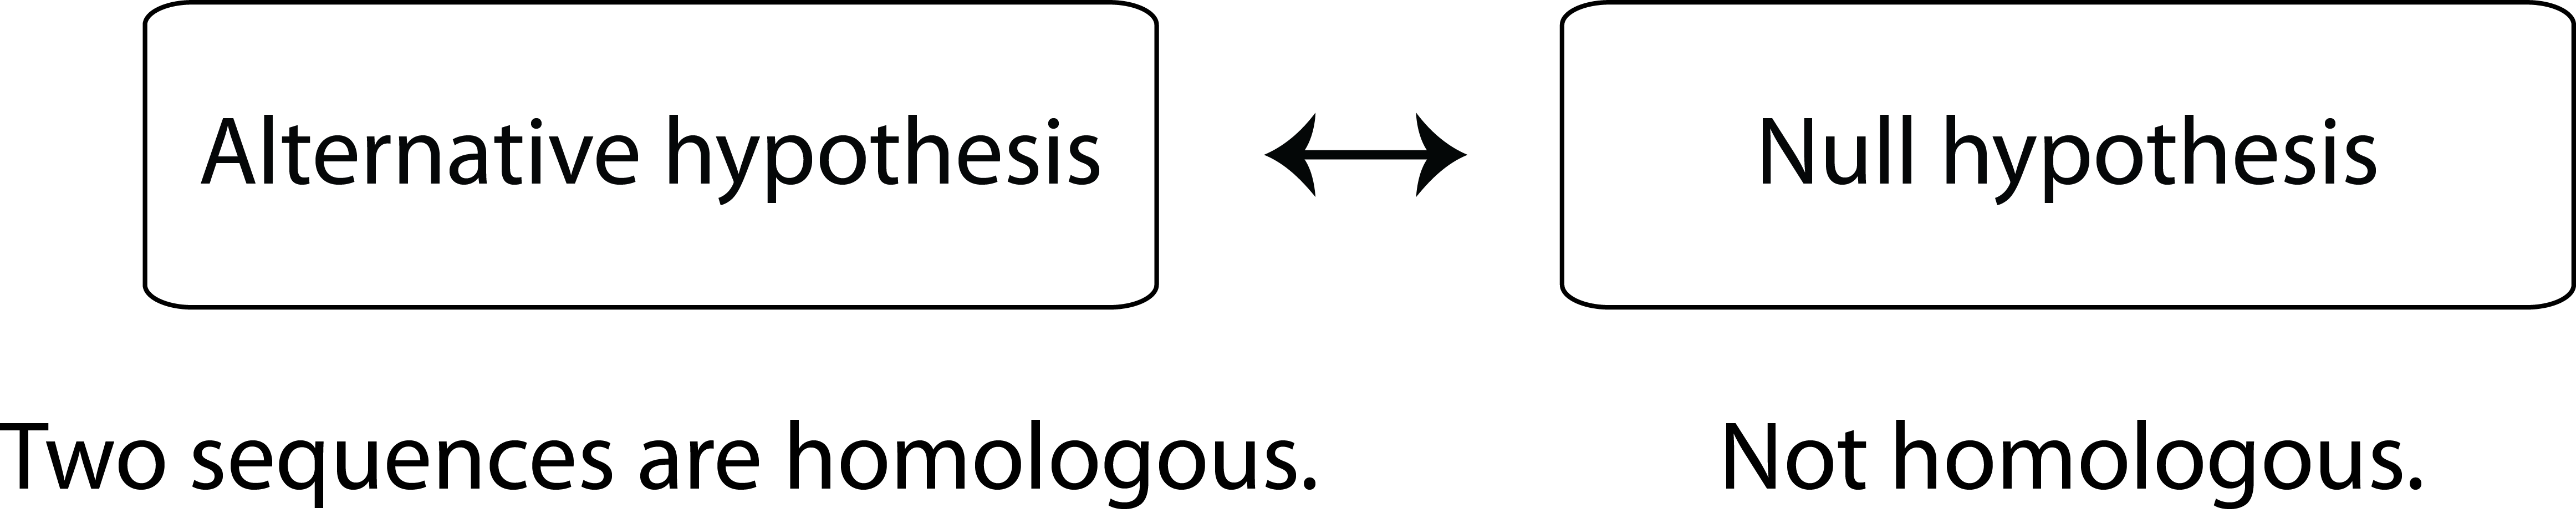
\includegraphics[width=0.6 \textwidth]{fig06/hypotheses.png}
  \caption{The null hypothesis and the alternative hypothesis}
\end{figure}

%
% P-value
%
\subsubsection*{P-value} 
``The p-value is defined as the probability of obtaining a result equal to or more extreme than what was actually observed, assuming that the null hypothesis is true.'' \\

\noindent
-- the p-value page on Wikipedia (\url{https://en.wikipedia.org/wiki/P-value})

%
% Significance level (\alpha)
%
\subsubsection*{Significance level ($\alpha$)} 
The significance level should be chosen to indicate strong/weak evidence against the null hypothesis. \\

\noindent
Significance levels 0.05 and 0.01 are often used in life sciences.
\begin{itemize}
\item Statistically significant: $\alpha$ = 0.05
\item Statistically highly significant: $\alpha$ = 0.01
\end{itemize}

%
% Common misunderstandings of p-value
%
\subsubsection*{Common misunderstandings of p-value} 
``The p-value is not the probability that the null hypothesis is true or the probability that the alternative hypothesis is false.'' \\

\noindent
-- the p-value page on Wikipedia (\url{https://en.wikipedia.org/wiki/P-value})

%
% Underlying (background) score distributions
%
\subsubsection*{Underlying (background) score distributions} 
\begin{table}[H]
\centering
\caption{Alignment methods and distributions}
\begin{tabular}{ll}
Method                     & Underlying distribution \\ \hline
Global alignment           & Unknown                 \\
Local alignment (ungapped) & Gumbel                 
\end{tabular}
\end{table}

\bigskip 

%\end{document}
